\documentclass[12pt]{article}
\usepackage{epsfig}
\usepackage{natbib}
\usepackage{amssymb,amsmath}
\usepackage{titletoc}
\usepackage{color}
\usepackage{graphicx}
\usepackage[toc,page]{appendix}

% HOW TO SET UP AN 8.5 x 11:
% http://www.pages.drexel.edu/~pyo22/students/latexRelated/latexTutorial.html
\topmargin -1.5cm        % read Lamport p.163
\oddsidemargin -0.04cm   % read Lamport p.163
\evensidemargin -0.04cm  % same as oddsidemargin but for left-hand pages
\textwidth 16.59cm
\textheight 21.94cm 
\parskip 7.2pt           % sets spacing between paragraphs
\parindent 0pt		     % sets leading space for paragraphs

%%%%%%%%%%%%%%%%%%%%%%%%%%%%%%%%%%%%%%%%%%%%%%%%%%%%%%%%%%%%%%%%%%%%%%
% set up formatting of python code
%
% to use insert python code, you can use
% \begin{python}
% ...
% \end{python}
\usepackage{listings}
\usepackage{color} % Used for syntax highlighting.
\usepackage{textcomp} % Used for syntax highlighting.

\renewcommand{\lstlistlistingname}{Code Listings}
\renewcommand{\lstlistingname}{Code Listing}
\definecolor{gray}{gray}{0.5}
\definecolor{key}{rgb}{0,0.5,0}
\lstnewenvironment{python}[1][]{
\lstset{
language=python,
basicstyle=\ttfamily\small,
otherkeywords={1, 2, 3, 4, 5, 6, 7, 8 ,9 , 0, -, =, +, [, ], (, ), \{, \}, :, *, !},
keywordstyle=\color{blue},
stringstyle=\color{red},
showstringspaces=false,
emph={class, pass, in, for, while, if, is, elif, else, not, and, or,
def, print, exec, break, continue, return},
emphstyle=\color{black}\bfseries,
emph={[2]True, False, None, self},
emphstyle=[2]\color{key},
emph={[3]from, import, as},
emphstyle=[3]\color{blue},
upquote=true,
morecomment=[s]{"""}{"""},
commentstyle=\color{gray}\slshape,
framexleftmargin=1mm, framextopmargin=1mm, frame=shadowbox,
rulesepcolor=\color{gray},#1
}}{}
%%%%%%%%%%%%%%%%%%%%%%%%%%%%%%%%%%%%%%%%%%%%%%%%%%%%%%%%%%%%%%%%%%%%%%

\definecolor{orange}{rgb}{1.00,0.65,0.00}
\def\arcsec{^{\prime\prime}}

\newcommand{\becker} { \textcolor{orange} {
\ensuremath{\blacksquare} {\bf AndyB:}  
\ensuremath{\blacksquare} } }

\newcommand{\simon} { \textcolor{red} {
\ensuremath{\bigstar} {\bf Simon:}  
\ensuremath{\bigstar} } }

\newcommand{\ajc} { \textcolor{blue} {
\ensuremath{\clubsuit} {\bf AndyC:}  
\ensuremath{\clubsuit} } }

\newcommand{\yusra} { \textcolor{cyan} {
\ensuremath{\diamondsuit} {\bf Yusra:}  
\ensuremath{\diamondsuit} } }

\newcommand{\russ} { \textcolor{green} {
\ensuremath{\natural} {\bf Russ:}  
\ensuremath{\natural} } }

%\titlecontents{subsection}[4.8em]{}{\contentslabel{2.4em}}{\hspace*{-2.8m}}{...}
%\titlecontents{subsubsection}[6.0em]{}{\contentslabel{2.4em}}{\hspace*{-2.8m}}{}

\author{Andrew Becker, Simon Krughoff, Andrew Connolly, Yusra AlSayyad, Russ Owen}
\title{Roadmap for Winter2013 Production}
\date{\today}

\begin{document}

\maketitle

The goal of late Winter2013 production is the testing of image
subtraction algorithms and the exercise of the {\tt ip\_diffim}
package.  The package may be utilized at 3 distinct portions of the
production pipeline: in the subtraction of Snaps for the rejection of
cosmic rays; in the matching of input images for a Psf--matched
template; and in the subtraction of this template from individual
science Exposures.

The input data will be simulated LSST images (ImSim); stretch goals
include application of the algorithms to SDSS Stripe82 data (S82).
The processing steps for the ImSim data include: application of the
Isr pipeline; combining the two Snaps in a Visit into a single
Exposure; calibration, detection, and measurement on the Exposure;
stacking of multiple Exposures into a Psf--matched template image;
subtraction of this template from single--epoch Exposures; detection,
measurement, and characterization of DiaSources that remain in the
difference image; and ingestion of these DiaSources into a MySQL
database.  The natural QA hooks are in the assessment of the
Psf--matched template, and in the purity of the DiaSource sample.  We
will focus on the following metrics to assess the production:
\begin{itemize}
\item rate of false positives
\item rate of missed detections
\item performance (computational and I/O)
\end{itemize}
This document outlines the details of each stage of production,
including estimates of compute time, and addresses the anticipated
Configs for each Task.

\clearpage
\tableofcontents
\clearpage

%%%%%%%

\clearpage 
\section{ImSim Input Data} \ajc

The sets of simulated images produced for Summer 2012 (which will be
the inputs for Winter 2013 late production) are described at \\{\tt
  http://dev.lsstcorp.org/trac/wiki/ImSim/Summer2012Plan}.  Processing
of SDSS Stripe82 data is a stretch goal for Winter 2013 production.

We wish to explore the capabilities of the image subtraction software
across the focal plane, and as a function of wavelength (both of the
sources and of the effective filter).  The former argues for
operations on (at a minimum) full quadrants of the focal plane, as
vignetting is known to attenuate the signal in the outer rafts.  The
latter argues for the analysis of observations in multiple passbands:
one band where chromatic effects are expected to be negligible
($i$--band) and one where the chromatic effects are expected to be
substantial ($g$--band).

The ImSim {\tt 5yr Run} simulated 2500 visits (full focal plane) of 5
adjacent fields over a 5-year period in the full suite of filters.
The simulations include both rotational and pointing dithering, and
the atmosphere includes no clouds or aerosols.  We will extract all of
the $i$--band data of the central field for a baseline study of the
image subtraction algorithms.  The $i$--band data will serve as a
reference set that maps out the underlying performance of the
algorithms in a regime where differential chromatic refraction (DCR)
within the bandpass is expected to be negligible.  The baseline spec
will be to generate a template image from the coaddition of the first
half of these data, with the appropriate cuts on conditions and
quality.  The second half of these data will be differenced with this
template, and the quality of the subtractions analyzed based on the
metrics above.  There are {\bf XX} $i$--band images of the central
field.

We will step through several sub--production runs to assess the
quality of the processing.  This includes sub--productions runs in the
following configurations:
\begin{itemize}
\item Images in $i$-band at low airmass to avoid the effects of DCR
\item Images in $i$-band over a short timescale to avoid proper motion effects
\end{itemize}

The second portion of production will move to the analysis of data in
the $g$--band, where DCR within the passband is expected at the scale
of the Psf.  This will inform future specifications for
color--dependent Psf--modeling and Psf--matching kernels.  There are
{\bf XX} $g$--band images of the central field.

Data will be prepared at various locations and stored at JHU with
images brought over as needed.  We can use standard grid copy tools
(gridftp, bbcp).  Before large runs start, the data will need to
staged at the compute center.  The estimated time of transfer is
(We'll need to benchmark this) demonstrated rate of {\bf XXX b/s} and
ImSim data volume of {\bf XXX GB} results in transfer time of {\bf
  XXX} days.  The registry generation time is ~10min per visit.  We
will need to solve the problem of how to point to the correct flat in
the registry given a rotator angle for the science image.  This has
not been done before.

We will be applying overscan correction, bias correction and flat
fielding to the ImSim data.  The dark current in the models is below
the level we need to worry about.  The flats will be normalized to a
global value.  The zeropoints should be consistent from chip to chip.
We {\it will} need rotation dependent flats due to vignetting.
Informed by John P. we should have flats in increments of 5 deg from 0
to 90.  Amps will be assembled in readout order such that the serial
transfer direction is along the x-axis of the image.

Master flats, darks, and biases will be produced by coadding 10
examples (each including 2 snaps).  We will not be simulating any time
dependent effects in the calibration products.

The spider introduces asymmetric vignetting.  This should be taken out
using flat fields produced with a variety of rotator angles.  Where
the effect is strongest, the angular dependence introduces scatter of
$\sim~5$\%.  Using flats generated at increments of 5 deg from 0 - 90
deg (18 master flats) should bring this below the nominal 1\% error
(although any remaining error will be systematic).

John will change the simulator to produce the chips in readout order
instead of camera coordinates so that the orientation of the eimage is
synchronized with the assembled calexps.

\subsection{Issues}

The calibration production will be non-trivial.  We'll need to make
registries for $\sim~200$ visits and process them at $\sim~$minutes
per chip.  The new calibration product tasks will make this much
easier.  Simon is working on said tasks.  As of Dec 11, 2 days worth
of work before it can be submitted for review.

%%%%%%%

\clearpage 
\section{CreateCalibrationProductsTask} \simon

%%%%%%%

\clearpage 
\section{ProcessCcdTask} \simon

\subsection{Input/Outputs}

Outputs will be:
\begin{itemize}
\item Metadata for ingest
\item Src for ingest
\item Calexp for input to {\tt ip\_diffim}
\item Background to add to Calexp for {\tt ip\_diffim}
\item Psf for Psf matching
\end{itemize}


\subsection{IsrTask} \simon

\subsection{SnapCombineTask} \becker

The baseline LSST observing plans defines a field ``visit'' as the
acquisition of two back--to--back images (called Snaps) and their
combination into a single visit Exposure.  The reason for this is to
reject cosmic rays that are fall outside the detection thresholds of
single--image CR rejection routines.  By subtracting the two snaps
(snap2 - snap1), CRs may be detected with either positive or negative
polarity, indicating a CR in the second or first snap, respectively.
These pixels will be masked, and the two snaps coadded into the final
visit Exposure.

There are two options to creating the image difference on which CRs
will be detected.  The first is to take a straight difference of the
two images.  This should suffice under the assumption of a fully
realized Psf and stable atmosphere, and of sufficient precision in the
telescope tracking over the 32 second visit window.  The second option
is to use a Psf--matching kernel to register both the shapes and/or
positions of the stars if any of the assumptions above fail.  A
disadvantage of this method is that, due to the convolution inherent
in Psf--matching, the shapes of the CRs will be distorted, potentially
making them more difficult to detect.

The outstanding issue driving the decision to use Psf--matching or not
is the amount of image motion between Snaps in the data.  The
amplitude of these shifts in the Winter2013 test data, determined
through manual source detection and matching, is {\bf XX}$\arcsec$.
This amplitude of shifts suggests that image registration techniques
will be necessary for Winter2013 processing. 

SnapCombine's SnapPsfMatchTask differs from ImagePsfMatchTask,
described in detail in Section~\ref{sec-imagedifftask}, in three major
ways to reflect the prior expectation that the images are not
significantly different.  First the spatial order of the matching
kernel is set to 0, indicating a constant matching kernel across the
image.  {\it For this reason it may be desirable to test out the
  delta--function kernel set in this environment}.  Second the size of
the matching kernel is approximately half the size of the
ImagePsfMatchTask matching kernel because shape is expected to be
approximately a delta function.  Finally, the sum--of--Gaussian basis
set is smaller (21 terms) than the default ImagePsfMatchTask set (31
terms).  The size of this basis set is a tuning parameter for the
production run.

After the snap difference Exposure is created, detection is next with
thresholdPolarity set to ``both''.  Measurement is then run on these
detections.  We currently do {\it not} have tools to reliably
distinguish true cosmic rays from the cores of bright stars.  Thus it
remains an open issue how aggressive we may be in masking out these
measurements.  We may compare the list of masked objects with the
known cosmic ray list, and with the known star list, to examine our
efficiency and purity.  These query tools do not exist yet.

The combined Exposure will have an exposure time equivalent to the sum
of the two input Snaps (i.e. this will {\it not} be an average image).
The FITS keywords that need to be modified in this process include:
{\bf XXX}.  The FITS keywords that will {\it not} be modified in this
process, but that do reflect metadata that are different between the
two Snaps, include : {\bf WCS}.  These features will be copied from
the first snap of the visit pair.  The FITS keywords that will {\it
  not} be modified in this process, and that are common between the
two Snaps, include: {\bf Filter}.

\subsection{Calibrate/Detect/Measure subTasks} \simon
The important parameters to consider are:
\begin{itemize} 
\item background grid size -- There are several of these in the config
  so we should understand what each one does
\item aperture size for aperture corrections -- the default is likely
  too small
\item deblending radius
\item galaxy shape parameters
\end{itemize}

\subsection{AstrometryTask} \simon

We already have a stars only reference catalog for the entire area
covered by the W13 ImSim area.  We will produce the galaxy catalog to
go along with this.  The reference catalog will contain the following
columns:

\begin{itemize}
\item id -- unique integer id of the object traceable back to the base catalogs
\item RA position of the object centroid in degrees
\item DEC position of the object centroid in degrees
\item {u,g,r,i,z,y} observed LSST magnitudes (in the mean sense for variable objects)
\item object class id (main sequence star, wd, bhb, etc.)
\item variability class (Agn, m-dwarf flare, RRly, etc. 0 if not variable)
\item galaxy position angle in degrees (do we measure these, or should we give these in both components)
\item galaxy semi-major axis 
\item galaxy semi-minor axis
\item bulge to total ratio
\item Agn to total ratio
\item disk to total ratio
\item Agn variability parameters (tau and SF\_{u,g,r,i,z,y})
\item A\_v reddening 
\end{itemize}

We will also need the reference catalog to be a function of time for
the time variable objects (brightness, position).  This has not been
done before.

\subsection{Issues}

We need to determine if this is a viable place to test out the
delta--function basis set.

We have not explored thoroughly the set of measurements that come from
the snap difference (efficiency and purity), and which are used to
mask pixels.

We do not know exactly how to obtain the list of cosmic rays that were
input (locations, shapes and amplitudes).

\subsection{New Developments}

We need code to reliably distinguish cosmic rays from the cores of
bright stars.

We need code to associate SnapCombine measurements with known cosmic
rays, and with the known locations of stars.

The reference catalog needs to have time--dependent entries.

\subsection{Tuning Parameters}

The type of basis set (sum--of--Gaussian or delta--function) used to
perform the SnapPsfMatchTask.

The size of the sum--of--Gaussian basis set if it is used.

\subsection{Metrics and Testing}

To determine how well we are detecting cosmic rays, we will
cross--match the list of masked pixels with the cosmic ray list, and
with the known star list.  We will calculate the efficiency () and
purity () of this sample as metrics to optimize.

\subsection{Tools}

%%%%%%%

\clearpage 
\section{MakeSkyMapTask} \russ

Creates a "sky map": a sky pixelization for coadds consisting of a collection of overlapping "tracts".
Each tract is, essentially, a very large exposure with its own WCS.
Tracts are subdivided into rectangular overlapping subregions called "patches".

The sky map we plan to use is DodecaSkyMap. It has 12 tracts arranged as the faces of a dodecahedron.
An alternative if we decide we want more smaller tracts is HealpixSkyMap which arranges
tracts as pixels in a HEALPix arrangement.

\subsection{Input/Outputs}

As for all tasks, specify an input and (optionally) output data repository.
makeSkyMap creates a sky map in the output repository.
A repository may have two sky maps: one for "deep" coadds and one for "goodSeeing" coadds.

\subsection{Issues}

DodecaSkyMap has large tracts which have significant distortion at the edges.
We don't believe this will be an issue for image differencing because the template is warped
to match the science exposure before subtracting. If it does prove to be a problem
we can switch to using HealpixSkyMap with smaller tracts.

SkyMap unpersistence has been a bit troublesome due to pickling pex_config fields.
When pex_config changes sometimes this breaks SkyMap unpersistence. We must fix this eventually.
I don't think it's a high priority, but we could try to fix it in time for late Winter2012 production.

\subsection{New Developments}

None. If we do decide to switch to HealpixSkyMap then we must make healpy an LSST package.
Healpy is self-contained other than needing cfitsio.

\subsection{Tuning Parameters}

These are the default parameters for LSSTSim:

\begin{python}
coaddName='deep' # or 'goodSeeing'
skyMap.name='dodeca'
skyMap.active.withTractsOnPoles=False
skyMap.active.projection='STG'
skyMap.active.patchInnerDimensions=[4000, 4000]
skyMap.active.pixelScale=0.2
skyMap.active.patchBorder=250
skyMap.active.tractOverlap=3.5
\end{python}

Image differencing should not be sensitive to these parameters.

The overlap between tracts may be larger than necessary, but the main effect of that
will be to slightly increase storage requirements of coadds and slightly increase
the time required to generate them. We will not see either effect in late Winter2012
because we are only working with a small region on the sky.

\subsection{Metrics and Testing}

No testing is required.

\subsection{Tools}

Skymap examples/plotSkyMap prints out useful information about a sky map and displays a 3d graph of it.

%%%%%%%

\clearpage 
\section{MakeCoaddTempExpTask} \yusra

The input images will be Psf--matched to a designed template Psf
before coaddition.  This Psf will be a circular double Gaussian
function, with the smaller of the Gaussians having the FWHM of the
{\bf XX}$^{th}$ percentile of the input images' FWHM.  The outer
Gaussian will have a FWHM of {\bf twice?} the central Gaussian, and
contribute {\bf $10\%$} of the total flux.

\subsection{Input/Outputs}

\subsection{WarpAndPsfMatchTask subTask} \becker
This subTask first undertakes the Psf--matching of the input {\tt
  calexp} to that desired for the Coadd.  It then astrometrically
warps this Psf--matched to the astrometric footprint of the Coadd.
The Psf--matching happens through the ModelPsfMatchTask subTask.  This
differs from ImagePsfMatchTask, described in detail in
Section~\ref{sec-imagedifftask}, in one major detail.  In this case,
the {\tt calexp's} {\it model} Psf is taken from the butler, and
compared to the idealized Psf that we wish to realize for the Coadd.
Each Psf is realized in a grid of $x,y$ positions around the {\tt
  calexp} to account for spatial variation of the {\tt calexp} Psf
(the Coadd Psf model will not be designed to vary).  This will be
entered into a KernelCandidate, which it itself entered into a
SpatialCellSet, and sent along to the fitting code where the
functionality is again the same as ImagePsfMatchTask.  Because the
concept of ``variance'' is nebulous when comparing model--to--model,
all sigma clipping is turned off and the variance is assumed to have a
constant weight.


There is trade--off in this process that needs to be explored in
detail.  First--off, we define the dimensions of the {\tt calexp} Psf
as $P \times P$, the FWHM of the Coadd Psf as $C$, and the dimensions
of the Psf--matching kernel as $K \times K$.  When fitting for the
matching Kernel, each Psf image gets convolved with the Kernel basis
functions, trimming $K//2$ pixels off of each side due to EDGE
effects.  Thus the final number of pixels we have to constrain the
Kernel coefficients are $(P-K) \times (P-K)$.  This means that as the
Kernel gets larger, the number of pixels we have to constrain the
solution gets smaller, and the solution may become unstable.
Providing tension in the other direction is that if the kernel
dimensions too small, to the extent that $P//2 < n \times C$ (i.e. its
smaller than say $n=3$ times the FWHM of the Psf you are matching to),
the kernel stamp is not large enough to capture all the power needed
to match to that large of a FWHM.  This ends up yielding ``boxy''
Psf--matched images.  Ultimately, we are limited by the dimensions of
the {\tt calexp} Psf model $P$, which in turn sets the maximum size of
the kernel such that $(P-K) \times (P-K)$ provides sufficient ability
to constrain all of the Kernel basis coefficients, which in turn sets
the size of the Psf we may match to ($C = P//2 / n$) without
sufficiently impacting the shapes of the stars.  This trade--off,
including the definitions of ``sufficient'' above, have not been
explored in thorough detail.

When choosing the desired FWHM of the Coadd, we will use the
distribution of FWHM of the input data.  Typically this comes from the
second or third quartile of the distribution; if we choose too narrow
of a FWHM to make a ``good seeing'' coadd, either we convolve the
smaller fraction of the data whose FWHM are less than the target, or
we deconvolve some fraction of the data.  The degree to which
deconvolution of the input images helps or hurts the salient qualities
of the coadd (depth, noise, and Psf) have not been fully explored in
detail.

\subsection{Issues}

The process of Psf--matching first, and then warping to the Coadd
footprint, may fail to represent the true shape of the Coadd Psf (in
pixel space) near the edges of tracts.

We have not explored the trade--offs between Psf dimensions, matching
kernel dimensions, and the FWHM of the Psf we may match to.

We do not have color-dependent Psfs.  This will be minimized by
analysis of $i$--band data, and explored in analysis of $g$--band
data.

We need to understand ``how much'' deconvolution the code can handle,
both in terms of the fraction of images that were deconvolved, and the
degree to which each of the images is deconvolved.

The {\tt meas\_mosaic}, which is a port of HSC's \"{u}ber cal, is
necessary to correct known deficiencies in LSST's {\tt meas\_astrom}
package.  This has proven necessary for creation of non--smeared
coadded images, reducing the RMS of the astrometric fit by a factor of
two.  This is leading to an additional systematic component equivalent
to {\bf XXX} in coadded images, and will vary spatially.

\subsection{New Developments}

Code to select from database

\subsection{Tuning Parameters}
We will need to test the following Psf--matching configs:
\begin{itemize}
\item Psf size (set in processCcd)
\item Psf grid 
\item Psf model functions
\item kernel size
\end{itemize}

\subsection{Metrics and Testing}

\subsection{Tools}

%%%%%%%

\clearpage 
\section{AssembleCoaddTask} \yusra

The coadded template image will be constructed using background
matching, as opposed to background subtraction.  The image subtraction
code will also be run using its own internal background--matching (of
template to science image) model, yielding a difference image with a
background level of 0.  Currently using a Chebyshev with order 3.

We need to make sure all necessary metadata ends up in the database.
This includes zeropoints, sky background, Psf FWHM.

\subsection{Input/Outputs}

\subsection{BackgroundMatchingTask} \yusra

\subsection{Issues}

Flux scaling (2-d spline)

\subsection{New Developments}
Spreading of Mask bits.  

How do we define the selection criteria, and select, input and
reference images from the database.

We need a tool that measures how well PSF matching to a model PSF
works. One source of such data is PSF-matched coadd temp exposures.

Flux scaling (2-d spline)

\subsection{Tuning Parameters}

\subsection{Metrics and Testing}

\subsection{Tools}

%%%%%%%

\clearpage 
\section{ProcessCoaddTask} \simon

To optimize the basis shapes matching the template image to a science
image, we require the Psf of the template image.  This level of
template processing also allows us to undertake QA to determine if the
realized shape of the Psf matches the specifications it was designed
to, if the astrometry of the template matches the SkyMap it was
designed to, and if there is any brightness dependence of the Psf by
looking at the measured brightness of reference catalog stars in the
template.  This essentially requires that we run calibrate, detection
and measurement on the template image, yielding at a minimum the {\tt
  Psf} and {\tt Source} products.

\subsection{Input/Outputs}

\subsection{Calibrate/Detect/Measure subTasks}

\subsection{Issues}

\subsection{New Developments}
Create zeropoint, Psf, and Wcs of coadd for QA, but do not overwrite
extant ones.

\subsection{Tuning Parameters}

\subsection{Metrics and Testing}

\subsection{Tools}
Means to compare fitted zeropoint, Psf, and Wcs of coadd with the
design specs.

%%%%%%%

\clearpage 
\section{ImageDifferenceTask \label{sec-imagedifftask}} \becker

The ImageDifferenceTask subtracts a template image that is
Psf--matched to the Psf of an input science image, from that science
image.  The residuals (the image difference, or difference image) will
contain only those objects that have varied in position or brightness
w.r.t. the template.  Detection and measurement will be run on the
difference image to characterize the residuals, both at positive and
negative polarity, and persisted as DiaSources.

In detail, an input {\tt calexp} has a bounding box from which the
Coadds will be queried.  The multiple SkyMap patches that overlap this
bounding box will be assembled into a single Exposure using the
ImageDifferenceTask.getTemplate method.  This mosaiced coadd
(a.k.a. the ``template'') is assumed to have a constant Psf and Calib
across patches; these values will be set from those in the first
overlapping patch.  The astrometric registration, and the
Psf--matching, will both happen on the template, leaving the {\tt
  calexp} pixels untouched.  This may in some cases result in
deconvolution of the template image.  The is a general sense that the
template may be deconvolved more reliably than the single--depth
images, due to its higher signal--to--noise, but this has not been
quantified.

Next the Task selects the objects to be used to Psf match the {\tt
  calexp} and template.  There are two options at the moment.  The
first involves use of a starSelectorRegistry.  This currently uses a
``second moment'' star selector to ensure that we only receive stars
in the list, but we may also adopt catalog--based selector that
queries a reference catalog for sources, and may be used as a
place--holder for a future specialized task that selects objects that
are non--variable and have negligible proper motion.  The second
option is to use native {\tt ip\_diffim} code that runs a very basic
detection algorithm and then sorts by integrated flux.  This code was
written long before starSelectorRegistries were implemented, and may
arguably be deprecated.  In both cases, objects with Mask bits set in
the Config (currently "EDGE" and "SAT") set are ignored.  We will run
selection on the source list from the template, as this should not
contain transient objects.  Another option is to instead run selection
on the source lists that come from measurement on the {\tt calexp} or
the {\tt coadd}, although the latter would have to be merged.

We next run the ImagePsfMatchTask.  This accepts the two Exposures,
the FWHM of their two Psfs, and the Source list as inputs.  The FWHM
will be used in a heuristic to determine the shape of the bases used
to model the Psf--matching kernel.  This heuristic needs to be tuned
on sample runs.  The overall number of bases becomes inflated by
multiplying each basis with a set of Hermite--polynomials.  The number
of bases ultimately used will be determined in pre--production by
using a principled means of deciding how much information each basis
contributes to the solution.  The Bayesian Information Criterion
provides one such means.

The internals of the ImagePsfMatchTask solve for $K(x,y)$ in the
equation $S(x,y) = (K \otimes T)(x,y)$, where $S$ is the science
calexp, $T$ is the template, and $K$ the Psf--matching kernel, by
performing a linear decomposition of $K$ such that $K(u,v) = \sum_i
a_i K_i(u,v)$.  The basis functions $K_i$ are decided using the
heuristic above; thus the challenge is to solve for $a_i$.
Additionally, the Psf--matching kernel is known to vary spatially
across the image, thus the general problem is to solve for $a_i(x,y)$.
This is accomplished by solving locally for $a_i$ at the positions
$x,y$ of each object returned by the object selector, and creating a
spatial model of these coefficients using a Chebyshev polynomial of
order $N$.  We thus have {\it two} solutions that describe the quality
of the Psf--match: using the original coefficients $a_i$; and using
the interpolated coefficients $a{'}_i$ that are derived from the
spatial model at $x,y$.  The distribution of residuals (mean and RMS
of: the diffim residuals normalized by the square root of the
variance) in each one of these KernelCandidates will be returned as
metadata.  Importantly, we will use the residuals of a control sample
of objects that are selected by the object selector, but not used in
the actual kernel fit, to determine the overall quality of the
difference image.

This process results in a subtracted Exposure (the difference image).
The detection planes of this image, inherited from the {\tt calexp}
will be wiped clean in preparation for detection and measurement.  The
Psf of the science image will be used to seed SourceDetectionTask,
with sources of both positive and negative polarity.
SourceDeblendTask is currently disabled in measurement.  Finally,
SourceMeasurementTask will be performed on the difference image source
catalog, using the aperture correction from the science image.  We
will run an instance of a DipoleChecker class to search for and flag
dipoles.  These will be persisted as DiaSources.  We require an
association of these DiaSources with the reference catalog {\it and}
the {\tt calexp} source catalog to assess where the sources are coming
from.  At this stage, this must be done manually.  DiaSources will be
written to the database in the {\tt WHAT} table, reference catalog
matches in the {\tt WHAT} table, and {\tt calexp} Source matches in
the {\tt WHAT} table.

\subsection{Input/Outputs}

Inputs are:
\begin{itemize}
\item A {\tt calexp} containing the science data, along with its {\tt
  Psf} and {\tt Wcs}
\item A set of Coadds that fully overlap the bounding box of the {\tt
  calexp}
\end{itemize}

Outputs are:
\begin{itemize}
\item Difference Exposure (data product; detection planes are set)
\item DiaSources (data product)
\item Psf--matched Image (metadata in pipeBase.Struct)
\item Psf--matching Kernel (metadata in pipeBase.Struct)
\item Background match (metadata in pipeBase.Struct)
\item KernelCellSet (metadata in pipeBase.Struct)
\end{itemize}

\subsection{ImagePsfMatchTask subTask}
As described above, this subTask controls the actual Psf-matching of
the {\tt calexp} and the template.  

\subsection{SourceDetectionTask subTask}
As described above, this subTask uses the Psf of the input {\tt
  calexp} to run detection on the difference Exposure.  The detection
Config will be set to search for objects of both positive and negative
polarity.  Estimation and re--estimation of the background will both
be disabled.

\subsection{SourceDeblendTask subTask}
As described above, this subTask is by default turned off.

\subsection{SourceMeasurementTask subTask}
As described above, this subTask performs measurement of the source
catalog returned by SourceDetectionTask.  It requires the aperture
correction of the {\tt calexp}.

\subsection{Issues}
We do not have color--dependent Psf--matching kernels,
e.g. $K(x,y,g-r)$, which are needed in the presence of differential
chromatic refraction.  This will impact the quality of the
Psf--matching happening in ImagePsfMatchTask, in particular for
objects of extreme color in the bluer passbands, and at high airmass.
We will first investigate the fitting of $K(x,y)$ in the absence of
DCR by operating on $i$--band data, and estimate the degradation in
the quality of the solution when going to $g$--band through the
control sample and debugging hooks.  Mitigation issues include
templates at different airmasses, but this also requires sets both East
and West of the meridian.

We need to assess the impact of objects with large proper motion on
the creation of the template, where the objects will appear elongated,
and on the residuals in the difference image, where such an apparition
will leave a complex dipole shape.  We will first investigate this by
creating templates from a finite window in time, and apply them to
images from a similar window.

We need to understand how to turn off the majority of the measurements
for the star selection, in the interest of speed.

We need to establish the minimum signal--to--noise of an object to be
used in Kernel fitting.

The number of sources that are detected in any given image determine
the complexity of the model that may be used to build a Psf--matching
kernel.  We need to decide if we are going to reduce the degree of the
spatial model based on the number of detected sources or not; this
means that the {\tt Config} will describe the heuristics used to
determine the spatial order of the models, and not the spatial order
of the models themselves.  This information needs to be persisted as
metadata if we choose to go this route.

We need to establish how much the template may be deconvolved in the
case that the science data have a narrower FWHM.  Alternately, we need
to understand the impacts of convolving the science image on the depth
we may detect to in the difference image.

\subsection{New Developments}
We need to evaluate the number of bases needed, using e.g. the
Bayesian Information Criterion, as a function of Psf FWHM and
variation.

We need to tune the heuristic that selects the shapes of the Gaussians
based on the FWHM of the {\tt calexp} and the template.

We need a piece of code to query the database, find the overlapping
tracts, and coadd them into a template.  A stub for this exists in
ImageDifferenceTask.getTemplate but has not been extensively tested.

\ajc Define the database query to specify the overlapping tracts that
will be used for template generation (stub exists in
ImageDifferenceTask.getTemplate)

We need to create a catalog--based selector to return objects for
Kernel modeling, if we choose to use this over the second--moment star
selector.

Do we use RHL's option to pre--convolve.

We need a dipole flag for the DiaSources.

We need source association for the DiaSources and the reference
catalog sources, and also with the {\tt calexp} Sources.

We need to exercise ingest of the DiaSources into MySQL.

We need to establish metrics and quality ranges to assess the goodness
of fit of the spatial kernel.

We need to implement these metrics in pipeQA.

Stretch goals : study of new bases, and Gaussian processes for
interpolation.

Turn into core chunks of work!
> - Develop Gaussian Processes based interpolation and evaluate against polynomial interpolation

\subsection{Tuning Parameters}
We need to decide on the object selection algorithm used to seed the
kernel fit.

We need to tune the heuristic that chooses the shapes and number of
basis function for the sum--of--Gaussian kernel basis.

The default for Winter2013 is to use Chebyshev polynomials for spatial
interpolation.  We need to use decide on the necessary spatial order
for this polynomial $N$.  A stretch goal will be to implement Gaussian
processes (kriging).

\subsection{Metrics and Testing}

Important metrics that will be exercised pre--production include: the
use of the BIC to determine the complexity of the kernel basis; an
examination of objects with large residuals in subtractions that we
expect to be nearly exact (what are their colors and proper motions).

In production our core metrics will include: what are the residuals of
a control sample of stars after application of the Psf--matching
kernel.

\subsection{Tools}
Several debugging hooks have been implemented in {\tt ip\_diffim} for
the visualization of the inputs and outputs to ImageDifferenceTask.
What remains to be done is to turn these into pipeQA tests; currently
no metrics querying the DiaSources exist.

%%%%%%%

\clearpage 
\section{Database Ingestion} \simon

\subsection{Input/Outputs}
\subsection{Issues}
\subsection{New Developments}
\subsection{Tuning Parameters}
\subsection{Metrics and Testing}
\subsection{Tools}

%%%%%%%

\clearpage 
\section{Summary} \becker

\subsection{Tall Poles}


%%%%%%%

\clearpage 
\section{Estimated Processing Times} \russ

\begin{table*}[h]
\small
\begin{center}
\caption{\label{tab-pars} Estimated Processing Times}
\begin{tabular}{lcccc}
\hline \hline
Task                          & Time/Unit     & Units        & Number of Units & Total Time\\
\hline
Build Registry                & 10 min        & Visit        & XXX             &           \\ 
ProcessCcdTask                & X min         & Ccd          & XXX             &           \\ % Sum of all 4 subtasks below
~~~~~~IsrTask                 & 1 min         & $\cdots$     & $\cdots$        &           \\
~~~~~~SnapCombineTask         &               & $\cdots$     & $\cdots$        &           \\
~~~~~~Calexp CDM              &               & $\cdots$     & $\cdots$        &           \\
~~~~~~AstrometryTask          &               & $\cdots$     & $\cdots$        &           \\
MakeSkyMapTask                & 10 sec        & Skymap       & 1               &           \\
MakeCoaddTempExpTask          &               & Visit-Patch  & XXX             &           \\
AssembleCoaddTask             &               & Patch        & XXX             &           \\   
ProcessCoaddTask              &               & Patch        & XXX             &           \\
ImageDifferenceTask           &               & Ccd          & XXX             &           \\
~~~~~~ImagePsfMatchTask       &               & $\cdots$     & $\cdots$        &           \\
~~~~~~SourceDetectionTask     &               & $\cdots$     & $\cdots$        &           \\
~~~~~~SourceMeasurementTask   &               & $\cdots$     & $\cdots$        &           \\
~~~~~~SourceDeblendTask       &               & $\cdots$     & $\cdots$        &           \\
\hline
Database Ingest               & 10$^{-X}$ sec & Rows         & XXX             &           \\
~~~~~~Calexp                  &               & Rows         & XXX             &           \\
~~~~~~Coadd                   &               & Rows         & XXX             &           \\
~~~~~~DiaSource               &               & Rows         & XXX             &           \\
\hline
\hline
\end{tabular}
\end{center}
\end{table*}

%%%%%%%
%%%%%%%
%%%%%%%

\clearpage 
\begin{appendices}
\section{Task Command lines and Configs}

\subsection{ProcessCcdTask}
\begin{python}
processCcd.py
\end{python}


\subsection{MakeSkyMapTask}
\begin{python}
makeSkyMap.py

--config
skyMap.name='dodeca'
skyMap.active.withTractsOnPoles=False
skyMap.active.projection='STG'
skyMap.active.patchInnerDimensions=4000,4000
skyMap.active.pixelScale=0.2
skyMap.active.patchBorder=250
skyMap.active.tractOverlap=3.5
\end{python}

\subsection{MakeCoaddTempExpTask} 
\begin{python}
makeCoaddTempExp.py
\end{python}

\subsection{AssembleCoaddTask} 
\begin{python}
assembleCoadd.py
\end{python}

\subsection{ProcessCoaddTask} 
\begin{python}
processCoadd.py
\end{python}

\subsection{ImageDifferenceTask} 
\begin{python}
imageDifference.py
\end{python}

\subsection{Database Ingestion} 
\begin{python}
$DATAREL_DIR/bin/ingest/ingestSources.py [lsstSim]
    ~becker/Winter2013/diffim_v0/tmpsdssdiff
    --host=lsst10.ncsa.illinois.edu 
    --database={yourDatabaseName} 
    --table={yourTableName}
    --dataset-type=goodSeeingDiff_src
    --id visit=873161311 raft=3,0 sensor=0,2
\end{python}
%$

%%%%%%%

\section{Flow Chart} 
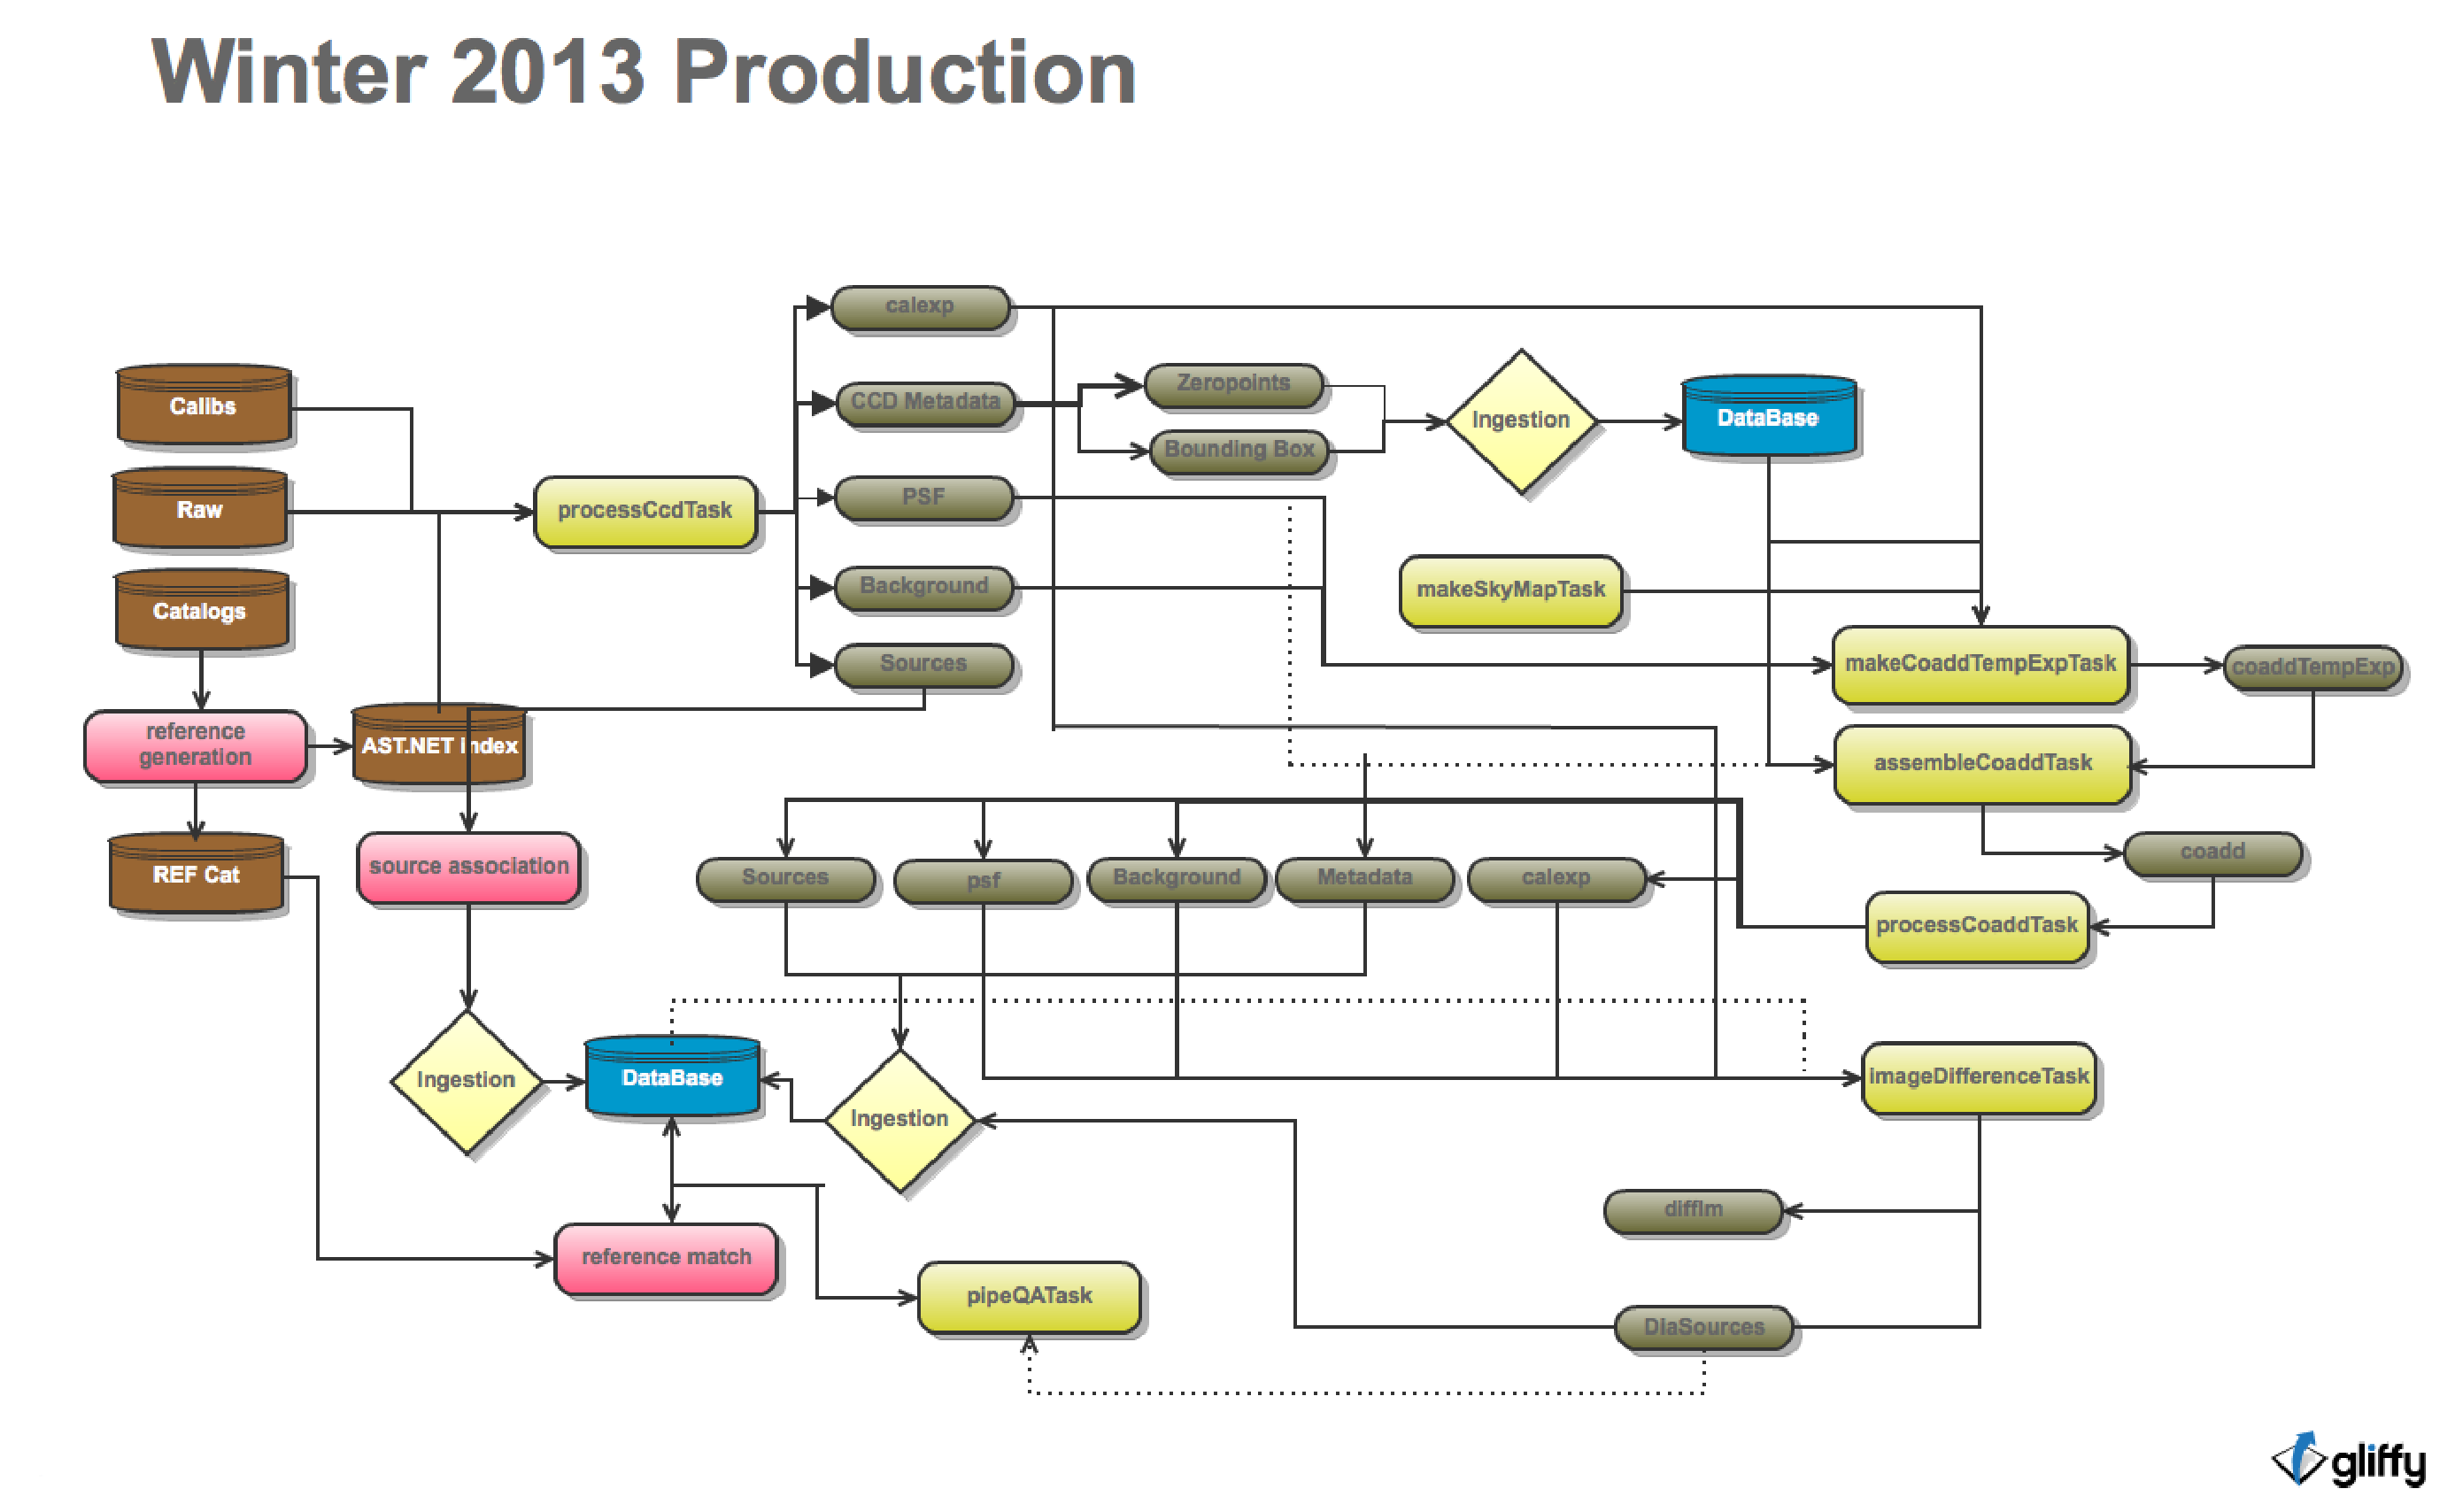
\includegraphics[height=0.7\textheight,angle=90]{flowChart.eps}

\clearpage 

\end{appendices}
%%%%%%%
%%%%%%%
%%%%%%%

\end{document}

















% Move the stuff below to above

%%%%%%%
\subsection{IsrTask (for ImSim)} \simon
Since there is no structure in the overscan, I do not believe we need
to do anything but the default for ISR.  That means overscan, bias,
flatfield, Cr interpolation, saturation and bad pixel corrections.
Right now the default for ImSim Isr is doDark=True.  This should be
fixed to reflect the fact that we no longer need dark correction with
the current model.

\subsubsection{What will be persisted}
In production we will only keep {\tt calexp}.  This means no {\tt
  postIsrCcd} will be persisted.  The Configs are automatically
persisted with the IsrTask.  Metadata to persist include: 
\begin{itemize}
\item nCR : the number of cosmic rays
\item median : the median of the calexp
\item image : 
\item gain : 
\item run time : 
\end{itemize}

\subsubsection{What is the processing time for ISR per Ccd}
The processing time is $\sim~1$ min per Ccd.

\subsubsection{What is the default Config for ISR}
\begin{python}
--config
doIsr=True
isr.doDark=False
\end{python}


\subsubsection{Which reference catalog will be used for the astrometry}

\subsubsection{Who will define it and create it from the sims}
This has been done based on the W13 surveys proposed on:
http://dev.lsstcorp.org/trac/wiki/ImSim/Summer2012Plan

\subsubsection{What depth is required for the reference catalog}
There is no reason to not go to 28$^{th}$ magnitude.  It's not that
big of an area.

\subsubsection{What format (and what processes) are required for the reference catalog}
This is very manual at the moment.  It would be nice to be able to
provide a CSV and schema to a routine that would produce both the
astrometry.net indexes and the match reach refObject.csv file.

\subsubsection{What metadata do we need to persist}
Metrics include: was the Wcs updated or did it default to the incoming
Wcs due to fitting failures; what is the RMS of the astrometric model
that was successfully fitted to the data.

\subsubsection{What is the default Config for AstrometryTask}
\begin{python}
--config
...
\end{python}




